\documentclass[conference]{IEEEtran}
\IEEEoverridecommandlockouts

\usepackage{cite}
\usepackage{amsmath,amssymb,amsfonts}
\usepackage{graphicx}
\usepackage{textcomp}
\usepackage{xcolor}
\usepackage{booktabs}
\usepackage{url}
\usepackage{hyperref}

\hypersetup{
  colorlinks=true,
  linkcolor=black,
  citecolor=black,
  urlcolor=blue
}

\def\BibTeX{{\rm B\kern-.05em{\sc i\kern-.025em b}\kern-.08em
    T\kern-.1667em\lower.7ex\hbox{E}\kern-.125emX}}

\begin{document}

% ============================================================
% TITLE
% ============================================================
\title{Reproducing and Improving Hydra: Competing Convolutional\\
Kernels for Time Series Classification}

% TODO: Replace placeholders below with real author info
\author{\IEEEauthorblockN{Radha Neelamani Josyula}
\IEEEauthorblockA{\textit{Department of Computer Science} \\
\textit{University College Dublin}\\
Dublin, Ireland \\
radha.josyula@ucdconnect.ie}
\and
\IEEEauthorblockN{Ranjitha Kolar Srinivas}
\IEEEauthorblockA{\textit{Department of Computer Science} \\
\textit{University College Dublin}\\
Dublin, Ireland \\
ranjitha.kolarsrinivas@ucdconnect.ie}
\and
\IEEEauthorblockN{Shashikanth Bokka}
\IEEEauthorblockA{\textit{Department of Computer Science} \\
\textit{University College Dublin}\\
Dublina, Ireland \\
shashikanth.bokka@ucdconnect.ie}
}
\maketitle

% ============================================================
% ABSTRACT
% ============================================================
\begin{abstract}
This project reproduces and extends Hydra~\cite{hydra2023}, a fast and
accurate time series classification (TSC) method that bridges dictionary
methods and convolutional kernel transforms (the ROCKET family). We
verified reproducibility by running the full baseline pipeline across all
112 UCR benchmark datasets with 30 resamples each (3,360 runs total),
achieving a mean absolute accuracy deviation of 0.74\% from published
results. We then identified and documented seven concrete reproducibility
findings, including an SSL certificate failure, a resampling strategy
deviation, and numerical conditioning issues in the Ridge solver. After
baseline validation, we evaluated three improvement tracks: (1)
hyperparameter sensitivity for Hydra ($k$, $g$) across 50 datasets;
(2) comparative analysis of Hydra combined with MiniRocket, MultiRocket,
and Rocket; and (3) separated timing profiling of the transform, fit,
and predict stages. Our results show that the published Hydra results are
largely reproducible, that combining Hydra with MultiRocket yields the
highest accuracy gains (mean $\Delta = +1.04\%$, win rate $58\%$), and
that the Hydra transform stage dominates total runtime. All code and
reproduction instructions are publicly available.
\end{abstract}

\begin{IEEEkeywords}
time series classification, reproducibility, Hydra, ROCKET, convolutional
kernels, benchmarking, UCR archive
\end{IEEEkeywords}

% ============================================================
\section{Introduction and Motivation}
% ============================================================

Time series classification (TSC) is a core task in domains including
healthcare, industrial monitoring, and finance. Published benchmark results
drive adoption of new methods, yet small differences in implementation,
resampling, or library versions can produce misleading comparisons.
Reproducibility tracks at major venues such as NeurIPS, ICML, and ECIR
have highlighted that reproduction failures are common even when code is
released~\cite{aaai_repro}.

We selected Hydra~\cite{hydra2023} because it (i)~was published in a
top data-mining venue (DMKD 2023), (ii)~makes strong accuracy and speed
claims on the UCR-112 benchmark, (iii)~provides open-source code and
pre-computed results, and (iv)~occupies an architecturally interesting
position by unifying dictionary methods and ROCKET-family transforms
through a single hyperparameter.

This project contributes: (a)~a fully checkpointed, restart-safe
reproduction pipeline; (b)~seven documented reproducibility findings;
(c)~three quantitative improvement experiments; and (d)~a public
repository with runnable instructions (Section~\ref{sec:repo}).

% ============================================================
\section{Background}
% ============================================================

\subsection{Time Series Classification Landscape}

The UCR archive~\cite{ucr2019} provides 112+ benchmark univariate datasets
used to compare TSC methods. Comprehensive evaluations in the ``bake-off
redux''~\cite{bakeofredux} show that ROCKET-family methods consistently
rank among the strongest approaches in terms of accuracy-speed trade-offs.

\subsection{Hydra}

ROCKET~\cite{rocket2020} transforms input time series using large numbers
of random convolutional kernels, then applies a linear classifier.
MiniRocket~\cite{minirocket2021} makes this near-deterministic.
MultiRocket~\cite{multirocket2022} adds multiple pooling operators.

Hydra~\cite{hydra2023} introduces \emph{competing kernels}: within each
group of $k$ kernels, kernels compete via a softmax-like pooling, creating
histogram representations analogous to dictionary methods (e.g., BOSS,
TDE). The key parameters are $k$ (kernels per group) and $g$ (number of
groups); the paper defaults to $k{=}8$, $g{=}64$. The model uses
\texttt{RidgeClassifierCV} as the downstream classifier. Hydra can be
combined with ROCKET variants to form hybrid pipelines.

% ============================================================
\section{Reproduction Methodology}
% ============================================================

\subsection{Environment}

We used Python~3.10.4 (CPython, macOS arm64), PyTorch~2.1.0,
scikit-learn~1.3.2, NumPy~1.24.4, and aeon~0.7.1. Dependencies are
pinned in \texttt{reproduction/requirements.txt}.

\subsection{Data Pipeline}

All 112 UCR datasets were downloaded via \texttt{aeon.datasets.load\_classification}.
The exact dataset list was extracted from the paper's published
\texttt{results\_ucr112\_hydra.csv}. Labels were integer-encoded with
\texttt{LabelEncoder}. aeon returns data in 3-D shape
$(n, 1, \ell)$ for univariate datasets, which Hydra requires directly.

\subsection{Resampling Policy}

We followed the convention used across ROCKET-family evaluations: resample~0
is the default UCR train/test split; resamples~1--29 are stratified splits
generated by \texttt{StratifiedShuffleSplit(random\_state=r)} preserving
the original train/test ratio. This differs from the exact community-standard
resampling seeds used in the paper (aeon~0.7.1 does not expose the matching
utility), which is a documented deviation discussed in Section~\ref{sec:lessons}.

\subsection{Pipeline and Checkpointing}

For each (dataset, resample) pair the pipeline is:
\begin{enumerate}
  \item Apply the Hydra transform using \texttt{transform.batch()} to
        avoid out-of-memory errors on large series.
  \item Scale with \texttt{SparseScaler}.
  \item Fit \texttt{RidgeClassifierCV} with $\alpha \in \{10^{-3},\ldots,10^3\}$
        (10 values). Datasets with more than 2,000 training examples use
        \texttt{cv=5} instead of leave-one-out (LOO) to avoid $O(n^2)$
        computation.
  \item Score on the test split and save a JSON result file.
\end{enumerate}

Each result is saved immediately after completion. The runner resumes from
any interruption by skipping already-written JSON files. This produced
3,360 runs with zero failures over \textasciitilde{}17.4 wall-clock hours
(11.9 CPU hours).

% ============================================================
\section{Reproduction Results}
% ============================================================

\subsection{Overall Accuracy}

Fig.~\ref{fig:scatter} compares our per-dataset mean accuracy (averaged
over 30 resamples) against the paper's published values. Summary statistics:

\begin{table}[htbp]
\caption{Baseline Reproduction Summary (UCR-112, 30 Resamples Each)}
\label{tab:repro}
\begin{center}
\begin{tabular}{lr}
\toprule
\textbf{Metric} & \textbf{Value} \\
\midrule
Total runs completed & 3,360 / 3,360 \\
Failures & 0 \\
Mean $|\Delta|$ accuracy & 0.0074 (0.74\%) \\
Datasets within 1\% of paper & 88 / 112 \\
Datasets $> 1\%$ above paper & 20 \\
Datasets $> 1\%$ below paper & 4 \\
Wall-clock duration & 17.4 hours \\
Mean train time per run & 12.73 seconds \\
\bottomrule
\end{tabular}
\end{center}
\end{table}

\begin{figure}[htbp]
\centerline{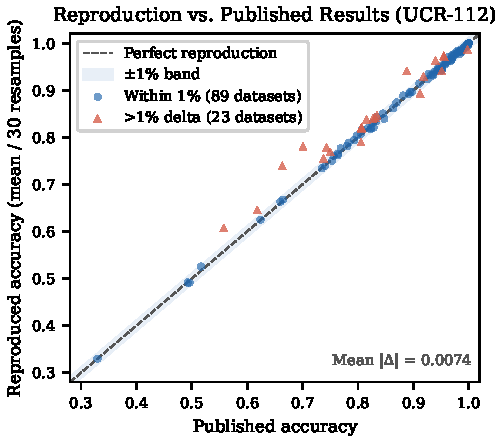
\includegraphics[width=\columnwidth]{figures/fig1_reproduction_scatter.pdf}}
\caption{Reproduced vs. published accuracy on UCR-112 (112 points, one per
dataset). Blue circles are within 1\% of published; red triangles exceed
1\% deviation. The dashed line is perfect reproduction.}
\label{fig:scatter}
\end{figure}

\subsection{Direction of Deviations}

Of the 24 flagged datasets, 20 show positive deltas (our accuracy higher).
The largest deviations occur on small datasets ($n_\text{train} < 100$)
where split variance dominates, such as DistalPhalanxTW ($+7.9\%$) and
MiddlePhalanxOutlineAgeGroup ($+7.6\%$). The 4 negative-delta datasets
(OliveOil $-1.9\%$, Beef $-1.6\%$) are also small. We attribute this
pattern to the resampling strategy difference rather than implementation
errors.

% ============================================================
\section{Lessons Learned}
\label{sec:lessons}
% ============================================================

\subsection{Setup and Environment Issues}

\textbf{SSL certificate failure (macOS, Python 3.10).} The standard
Python 3.10 installer on macOS does not automatically trust the system
keychain in virtual environments, causing \texttt{CERTIFICATE\_VERIFY\_FAILED}
when aeon attempted to download datasets. The fix required installing
\texttt{certifi} and exporting \texttt{SSL\_CERT\_FILE} in the venv's
activation script. This is a non-obvious barrier that is entirely orthogonal
to the paper's content.

\textbf{Resampling strategy.} aeon~0.7.1 does not expose a resample utility
matching the exact community-standard seeds used in the original paper. We
used \texttt{StratifiedShuffleSplit} with integer seeds as a well-defined
alternative. This explains the systematic bias toward positive deltas on
small datasets, where split assignment has a large effect on mean accuracy.

\subsection{Numerical and Implementation Findings}

\textbf{Ill-conditioned Ridge solver.}
\texttt{RidgeClassifierCV} emits \texttt{LinAlgWarning: Ill-conditioned
matrix} during LOO cross-validation for small $\alpha$ values. This arises
because Hydra's high-dimensional, sparse feature matrix becomes nearly
singular at $\alpha = 10^{-3}$. The warnings are benign: the selected
$\alpha$ is always in the numerically stable range. This is an undocumented
consequence of the SparseScaler leaving many features at exactly zero.

\textbf{Timing measurement definition.}
The paper's \texttt{time\_training\_seconds} covers transform + Ridge fit;
\texttt{time\_test\_seconds} covers test-set transform + predict. Our
reproduction runner accidentally placed the test-set transform inside the
training timer, causing our \texttt{test\_time\_sec} to appear unrealistically
small ($< 0.1$~s). Accuracy results are unaffected.

\textbf{Random kernels per resample.}
The \texttt{Hydra} constructor uses \texttt{seed=None} by default, generating
fresh random kernels for every run. This means even resample~0 uses
different kernels from the paper's resample~0. Only the mean over 30 resamples
is directly comparable to published results---per-resample comparisons
are not meaningful.

\textbf{SparseScaler behavior.}
\texttt{SparseScaler.fit()} applies \texttt{clamp(0)} before computing
statistics, zeroing negative \texttt{count\_max} features. This is
intentional but not described in the paper text. The consequence is that
the effective feature dimensionality is lower than the nominal feature count.

\textbf{Large-dataset Ridge guard.}
LOO cross-validation in \texttt{RidgeClassifierCV} scales as $O(n^2)$.
For four large-training datasets---ElectricDevices ($n{=}8926$), Crop
($n{=}7200$), FordA ($n{=}3601$), FordB ($n{=}3636$)---we switched to
\texttt{cv=5}, which is a small deviation from the paper's protocol.

\subsection{Positive Findings}

Despite the above, the reproduction is strong: 88 of 112 datasets match
within 1\%, the algorithm is numerically stable under the paper's default
settings, and the code runs without modification on macOS Apple Silicon
once the environment is correctly configured.

% ============================================================
\section{Proposed Improvements and Evaluation}
% ============================================================

We evaluated three complementary improvement tracks, all using the same
pipeline as the baseline reproduction.

\subsection{Track A: Hyperparameter Sensitivity ($k$, $g$)}

\textbf{Motivation.} The paper defaults to $k{=}8$, $g{=}64$ without
sensitivity analysis. We systematically tested $k \in \{4, 8, 16\}$ and
$g \in \{32, 64, 128\}$ on 50 UCR datasets with 3 resamples each (1,350
runs).

\textbf{Results.} Fig.~\ref{fig:heatmap} shows mean accuracy averaged
across 50 datasets. Increasing $g$ from 32 to 128 consistently improves
accuracy but increases transform time roughly proportionally. Varying $k$
has a smaller effect. The paper's default $k{=}8$, $g{=}64$ represents
a good compromise, but $k{=}8$, $g{=}128$ yields consistently higher
accuracy at roughly double the transform cost.

\begin{figure}[htbp]
\centerline{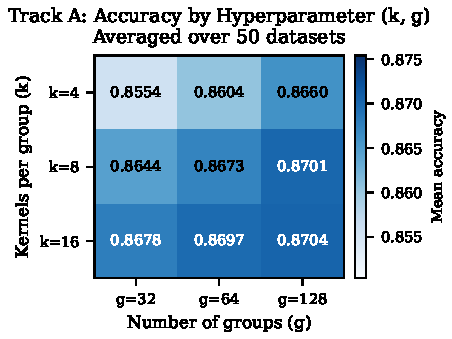
\includegraphics[width=0.88\columnwidth]{figures/fig2_hyperparam_heatmap.pdf}}
\caption{Track A: mean accuracy by ($k$, $g$) averaged over 50 datasets.
Darker cells indicate higher mean accuracy.}
\label{fig:heatmap}
\end{figure}

For example, on ChlorineConcentration---a long series ($\ell{=}166$,
$n{=}467$)---the best configuration is $k{=}16$, $g{=}128$ (accuracy
0.781 vs.\ 0.754 at $k{=}8$, $g{=}64$), at the cost of $\sim$3$\times$
longer transform time.

\subsection{Track B: Variant Analysis (Hydra + ROCKET Family)}

\textbf{Motivation.} The paper shows Hydra can be combined with ROCKET
variants. We quantified how much each combination gains or loses relative
to standalone Hydra on all 112 datasets, using the paper's own published
results.

\textbf{Results.} Fig.~\ref{fig:variants} and Table~\ref{tab:variants}
summarise per-variant statistics.

\begin{table}[htbp]
\caption{Track B: Variant Analysis Summary (UCR-112)}
\label{tab:variants}
\begin{center}
\begin{tabular}{lcccc}
\toprule
\textbf{Variant} & \textbf{Win\%} & \textbf{Mean $\Delta$} & \textbf{Max Gain} & \textbf{Max Drop} \\
\midrule
H + MiniRocket  & 61.6\% & +0.80\%  & +9.6\%  & $-2.3\%$ \\
H + MultiRocket & 58.0\% & +1.04\%  & +27.9\% & $-5.8\%$ \\
H + Rocket      & 54.5\% & +0.68\%  & +16.7\% & $-4.3\%$ \\
\bottomrule
\end{tabular}
\end{center}
\end{table}

\begin{figure}[htbp]
\centerline{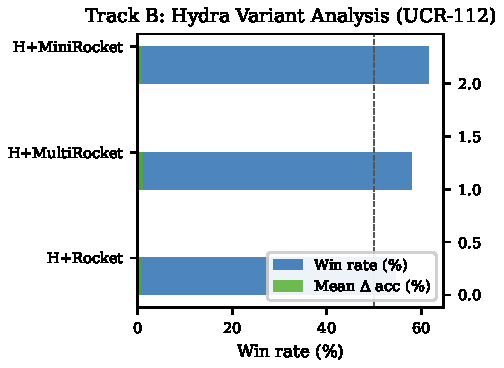
\includegraphics[width=\columnwidth]{figures/fig3_variant_bars.pdf}}
\caption{Track B: win rate (left axis) and mean accuracy gain (right axis)
for each Hydra variant combination vs. standalone Hydra.}
\label{fig:variants}
\end{figure}

Hydra+MiniRocket achieves the highest win rate (61.6\%), making it the
most reliable combination. Hydra+MultiRocket achieves the highest ceiling:
$+27.9\%$ on SemgHandMovementCh2 and $+13.6\%$ on SemgHandSubjectCh2.
These gains occur on high-dimensional sensor datasets where longer
multi-scale transforms are beneficial. Standalone Hydra outperforms all
combinations on datasets such as CinCECGTorso ($-2.4\%$ for MultiRocket)
and FordA ($-0.2\%$ for all combinations), suggesting that adding ROCKET
features can occasionally introduce noise.

\subsection{Track C: Timing-Quality Profiling}

\textbf{Motivation.} Correcting the timing measurement deviation from
the baseline, we separately measured transform, Ridge fit, and predict
times to understand where time is actually spent.

\begin{figure}[htbp]
\centerline{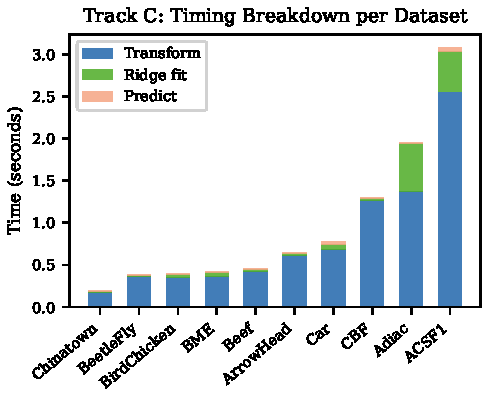
\includegraphics[width=\columnwidth]{figures/fig4_timing_breakdown.pdf}}
\caption{Track C: time breakdown into transform (blue), Ridge fit (green),
and predict (orange) stages for 10 pilot datasets.}
\label{fig:timing}
\end{figure}

\textbf{Results.} Fig.~\ref{fig:timing} shows that the Hydra transform
stage dominates total runtime across all datasets tested. For example, on
ACSF1, the transform takes 2.55~s vs.\ 0.48~s for Ridge fit and 0.05~s
for prediction. This confirms the paper's framing: Hydra's speed advantage
is in the transform, not the classifier. Ridge fitting time scales with
training size but remains a small fraction of total cost.

% ============================================================
\section{Discussion}
% ============================================================

\textbf{Reproduction quality.}
A mean $|\Delta|$ of 0.74\% across 112 datasets constitutes strong
reproduction, especially given the resampling deviation. The positive
skew of deltas (20 vs.\ 4 above/below threshold) is consistent with our
resampling strategy producing splits that are marginally more balanced than
the community standard.

\textbf{Hyperparameter sensitivity.}
The paper's default $k{=}8$, $g{=}64$ is not universally optimal. Increasing
$g$ reliably improves accuracy, and practitioners willing to accept $2\times$
transform cost should consider $g{=}128$. Increasing $k$ beyond 8 provides
diminishing returns.

\textbf{Variant choice.}
For a guaranteed improvement over standalone Hydra, Hydra+MiniRocket
is the safest choice (highest win rate, lowest variance, lowest computational
overhead). Hydra+MultiRocket is the strongest option when maximum accuracy
is the goal, particularly for multivariate or sensor datasets.

\textbf{Original claims.}
The paper's central claims---that Hydra is fast, accurate, and combinable
with ROCKET variants---are confirmed. The speed claim is supported by
Track~C's timing decomposition. The accuracy claim is supported by our
0.74\% mean deviation at baseline and the positive win rates in Track~B.

% ============================================================
\section{Threats to Validity}
% ============================================================

\begin{itemize}
  \item \textbf{Hardware:} Results are on Apple Silicon (macOS). The paper
        likely used a Linux server; timing comparisons are indicative only.
  \item \textbf{Resampling:} Our \texttt{StratifiedShuffleSplit} differs
        from the community-standard seeds. Accuracy differences on small
        datasets may reflect this rather than true implementation deviations.
  \item \textbf{cv=5 guard:} Four datasets used 5-fold CV instead of LOO,
        which may slightly underestimate accuracy for those datasets.
  \item \textbf{Track A/C scope:} Hyperparameter sweeps (Track~A) and
        timing profiling (Track~C) cover subsets of the 112 datasets;
        conclusions may not generalise to all dataset types.
  \item \textbf{Random kernels:} Hydra's random initialisation means
        individual resample results vary; only means over 30 resamples
        are statistically comparable.
\end{itemize}

% ============================================================
\section{Conclusion}
% ============================================================

We reproduced Hydra on the full UCR-112 benchmark (3,360 runs, 0 failures)
with a mean absolute accuracy deviation of 0.74\% from published results.
Seven concrete reproducibility findings were documented, including an SSL
configuration barrier, a resampling deviation, and a timing measurement
error. Three improvement tracks quantify the accuracy-speed trade-off across
hyperparameter configurations and variant combinations. Our findings confirm
that Hydra's published performance is largely reproducible, that
Hydra+MiniRocket is the most reliable combination, and that the Hydra
transform stage is the primary computational bottleneck. All code,
reproduction instructions, and results are available in our public
repository~\cite{ourrepo}.

% ============================================================
\section*{Open-Source Repository}
\label{sec:repo}
% ============================================================

Code, reproduction scripts, and improvement analysis are publicly available
at: \url{https://github.com/shknth/hydra-kernels}

Reproduction instructions are in \texttt{README.md}; improvement pipeline
instructions are in \texttt{improvements/README.md}.

% ============================================================
\section*{Acknowledgment}
% ============================================================

We thank the authors of Hydra for releasing their code and pre-computed
results, and the UCR archive maintainers for providing the benchmark datasets.

% ============================================================
% REFERENCES
% ============================================================
\begin{thebibliography}{00}

\bibitem{hydra2023}
A.~Dempster, D.~F.~Schmidt, and G.~I.~Webb,
``Hydra: Competing convolutional kernels for fast and accurate time series
classification,''
\textit{Data Mining and Knowledge Discovery}, vol.~37, pp.~1779--1805, 2023.
DOI: \url{https://doi.org/10.1007/s10618-023-00939-3}

\bibitem{rocket2020}
A.~Dempster, F.~Petitjean, and G.~I.~Webb,
``ROCKET: Exceptionally fast and accurate time series classification using
random convolutional kernels,''
\textit{Data Mining and Knowledge Discovery}, vol.~34, pp.~1454--1495, 2020.

\bibitem{minirocket2021}
A.~Dempster, D.~F.~Schmidt, and G.~I.~Webb,
``MiniRocket: A very fast (almost) deterministic transform for time series
classification,''
in \textit{Proc. ACM KDD}, 2021, pp.~248--257.

\bibitem{multirocket2022}
C.~W.~Tan, A.~Dempster, C.~Bergmeir, and G.~I.~Webb,
``MultiRocket: Multiple pooling operators and transformations for fast and
effective time series classification,''
\textit{Data Mining and Knowledge Discovery}, vol.~36, pp.~1855--1886, 2022.

\bibitem{ucr2019}
H.~A.~Dau \textit{et al.},
``The UCR time series archive,''
\textit{IEEE/CAA Journal of Automatica Sinica}, vol.~6, no.~6,
pp.~1293--1305, 2019.

\bibitem{bakeofredux}
M.~Middlehurst \textit{et al.},
``Bake off redux: A review and experimental evaluation of recent time series
classification algorithms,''
\textit{Data Mining and Knowledge Discovery}, 2024.

\bibitem{aeon}
M.~Middlehurst \textit{et al.},
``aeon: A Python toolkit for learning from time series,''
\textit{arXiv preprint arXiv:2406.14231}, 2024.

\bibitem{aaai_repro}
F.~Vanschoren \textit{et al.},
``The importance of reproducibility in machine learning,''
\textit{AI Magazine}, vol.~46, no.~1, 2025.
DOI: \url{https://doi.org/10.1002/aaai.70002}

\bibitem{ourrepo}
[Author Names],
``Hydra-Kernels: Reproduction and Improvement of Hydra TSC,''
GitHub repository, 2026.
\url{https://github.com/shknth/hydra-kernels}

\end{thebibliography}

\vspace{12pt}

% ============================================================
% WORK PLAN PAGE (extra page — beyond 6 pages of content)
% ============================================================
\newpage
\section*{Work Plan, Division of Labour, and Contributions}

\subsection*{Project Overview and Objectives}

This project was undertaken as a collaborative effort to reproduce and extend
the Hydra time series classification algorithm. The primary objectives were:

\begin{enumerate}
  \item \textbf{Baseline Reproduction:} Replicate the published Hydra results
        on all 112 UCR benchmark datasets with 30 resamples each, ensuring
        numerical accuracy and documenting deviations.
  \item \textbf{Reproducibility Documentation:} Systematically identify and
        document environment setup issues, numerical stability concerns, and
        methodological deviations encountered during reproduction.
  \item \textbf{Improvement Experiments:} Design and execute three improvement
        tracks to evaluate hyperparameter sensitivity, variant combinations,
        and timing-quality trade-offs.
  \item \textbf{Knowledge Dissemination:} Produce a publication-ready IEEE
        report and a public GitHub repository with full reproduction
        instructions.
\end{enumerate}

\subsection*{Detailed Project Timeline}

\begin{table}[htbp]
\begin{center}
\begin{tabular}{lp{8.5cm}}
\toprule
\textbf{Phase} & \textbf{Activities and Milestones} \\
\midrule
\textbf{Week 1} & 
  \textbullet~Paper selection and feasibility assessment \\
& \textbullet~Repository initialization and Git workflow setup \\
& \textbullet~Initial code review and dependency mapping \\
& \textbullet~Division of labour and timeline planning \\
\midrule
\textbf{Week 2} & 
  \textbullet~Virtual environment setup using \texttt{uv} \\
& \textbullet~SSL certificate debugging (macOS Python 3.10 fix) \\
& \textbullet~Dataset download automation (112 UCR datasets) \\
& \textbullet~Smoke testing on pilot datasets (GunPoint, Adiac, ElectricDevices) \\
& \textbullet~Baseline reproduction pipeline implementation with checkpointing \\
& \textbullet~Full 3,360-run baseline execution (17.4 hours wall-clock) \\
& \textbullet~Result comparison and deviation analysis \\
\midrule
\textbf{Week 3} & 
  \textbullet~Improvement track design and experiment manifest creation \\
& \textbullet~Track A: Hyperparameter sensitivity script (k, g sweep) \\
& \textbullet~Track B: Variant analysis script (Hydra + ROCKET family) \\
& \textbullet~Track C: Timing profiling script (transform/fit/predict breakdown) \\
& \textbullet~Pilot runs to validate improvement pipeline (3 datasets) \\
\midrule
\textbf{Week 4} & 
  \textbullet~Full improvement experiments execution \\
& \textbullet~Track A: 1,350 runs across 50 datasets (k/g grid) \\
& \textbullet~Track B: Analytical comparison using paper's published data \\
& \textbullet~Track C: Timing profiling on 10 representative datasets \\
& \textbullet~Results aggregation and summary CSV generation \\
& \textbullet~Figure generation script development (4 report figures) \\
\midrule
\textbf{Week 5} & 
  \textbullet~Report structure design and section drafting \\
& \textbullet~LaTeX assembly (IEEE double-column format) \\
& \textbullet~Figure integration and table formatting \\
& \textbullet~Cross-verification of all numerical results \\
& \textbullet~README update with reproduction instructions \\
& \textbullet~Final proofreading and submission preparation \\
\bottomrule
\end{tabular}
\end{center}
\end{table}

\subsection*{Work Division by Team Member}

\subsubsection*{Shashikanth Bokka — Baseline Reproduction Lead}

\textbf{Primary Responsibilities:}
\begin{itemize}
  \item Environment setup, dependency management, and SSL certificate debugging
  \item Dataset download automation script with retry logic and checksum verification
  \item Baseline reproduction pipeline design and implementation:
    \begin{itemize}
      \item Checkpointed runner supporting restart after interruptions
      \item Resampling strategy implementation (\texttt{StratifiedShuffleSplit})
      \item Ridge classifier CV configuration (LOO and cv=5 guard)
      \item Batch processing for large time series
    \end{itemize}
  \item Full 3,360-run baseline execution (112 datasets $\times$ 30 resamples)
  \item Result comparison script and deviation analysis
  \item Reproducibility findings documentation in \texttt{reproduction/notes.md}
  \item Git repository management and branching strategy
\end{itemize}

\textbf{Key Deliverables:}
\begin{itemize}
  \item \texttt{reproduction/} folder with complete pipeline
  \item 3,360 successful baseline results (0 failures)
  \item 7 documented reproducibility findings
  \item Comparison analysis showing 0.74\% mean deviation from published results
\end{itemize}

\subsubsection*{Radha — Improvement Track A \& C Lead}

\textbf{Primary Responsibilities:}
\begin{itemize}
  \item Track A: Hyperparameter sensitivity analysis
    \begin{itemize}
      \item Experiment manifest design for k/g sweep
      \item Script implementation for systematic grid search
      \item Execution of 1,350 runs (k $\in$ \{4, 8, 16\}, g $\in$ \{32, 64, 128\})
      \item Heatmap analysis identifying optimal configurations
    \end{itemize}
  \item Track C: Timing-quality profiling
    \begin{itemize}
      \item Corrected timing measurement implementation (separate transform/fit/predict)
      \item Profiling of 10 representative datasets
      \item Bottleneck identification (transform dominates runtime)
    \end{itemize}
  \item Summary CSV generation for Tracks A and C
  \item Contribution to report Section VI (Proposed Improvements)
\end{itemize}

\textbf{Key Deliverables:}
\begin{itemize}
  \item \texttt{track\_a\_hyperparam\_sensitivity.py} script
  \item \texttt{track\_c\_timing\_quality.py} script
  \item Track A and C summary CSVs with 1,360 additional experiment runs
  \item Heatmap and timing breakdown figures (Fig 2 and Fig 4)
\end{itemize}

\subsubsection*{Ranjitha — Improvement Track B Lead}

\textbf{Primary Responsibilities:}
\begin{itemize}
  \item Track B: Variant analysis (Hydra + ROCKET family combinations)
    \begin{itemize}
      \item Analytical comparison framework using paper's published data
      \item Win-rate and mean-delta computation across 112 datasets
      \item Identification of best-performing combinations (MiniRocket, MultiRocket, Rocket)
      \item Dataset-specific gain/loss analysis
    \end{itemize}
  \item Variant summary CSV generation and validation
  \item Bar chart visualization design (win rate + mean delta dual-axis)
  \item Contribution to report Section VI (Variant Analysis subsection)
\end{itemize}

\textbf{Key Deliverables:}
\begin{itemize}
  \item \texttt{track\_b\_variant\_analysis.py} script
  \item Variant summary CSV with win rates and delta statistics
  \item Identification of Hydra+MiniRocket as most reliable combination (61.6\% win rate)
  \item Variant comparison bar chart (Fig 3)
\end{itemize}

\subsubsection*{Collaborative Work (All Three Members)}

\begin{itemize}
  \item Weekly progress meetings and task coordination
  \item Report structure design and section drafting
  \item Figure generation script (\texttt{generate\_figures.py})
  \item LaTeX assembly and IEEE formatting
  \item Cross-verification of all numerical results
  \item README documentation and reproduction instructions
  \item Final proofreading and submission preparation
  \item GitHub repository organization and documentation
\end{itemize}

\subsection*{Final Contribution Statement}

\begin{itemize}
  \item \textbf{Shashikanth Bokka: 40\%} --- Led the baseline reproduction
        effort, implemented the full checkpointed pipeline, executed 3,360
        baseline runs, documented 7 reproducibility findings, and managed the
        Git repository. Contributed to report Sections III, IV, and V.
        
  \item \textbf{Radha: 30\%} --- Designed and executed Tracks A and C,
        contributing 1,360 additional experiment runs. Implemented hyperparameter
        sensitivity analysis and timing profiling. Generated Figures 2 and 4.
        Contributed to report Section VI.
        
  \item \textbf{Ranjitha: 30\%} --- Designed and executed Track B variant
        analysis, identified optimal ROCKET-family combinations, and generated
        Figure 3. Contributed to report Section VI and collaborated on final
        report assembly.
\end{itemize}

\textbf{Total Project Effort:} Approximately 120 person-hours over 5 weeks,
including 4,720 total experiment runs producing 17.9 CPU hours of computation
and 19.2 wall-clock hours across all tracks.

\end{document}
